%%%%%%%%%%%%%%%%%%%%%%%%%%%%%%%%%%%%%%%%%
% Beamer Presentation
% LaTeX Template
% Version 1.0 (10/11/12)
%
% This template has been downloaded from:
% http://www.LaTeXTemplates.com
%
% License:
% CC BY-NC-SA 3.0 (http://creativecommons.org/licenses/by-nc-sa/3.0/)
%
%%%%%%%%%%%%%%%%%%%%%%%%%%%%%%%%%%%%%%%%%

%----------------------------------------------------------------------------------------
%	PACKAGES AND THEMES
%----------------------------------------------------------------------------------------

\documentclass[xcolor=table]{beamer}

\usepackage{tikz}
\setbeamertemplate{background canvas}{\begin{tikzpicture}\node[opacity=.3]{
\includegraphics
		[width=\paperwidth]{imagenes/background2.png}};\end{tikzpicture}}

%\setbeamertemplate{background}
%{
\includegraphics[width=\paperwidth,height=\paperheight,keepaspectratio]{imagenes/background2.png}}

\mode<presentation> {

% The Beamer class comes with a number of default slide themes
% which change the colors and layouts of slides. Below this is a list
% of all the themes, uncomment each in turn to see what they look like.

%\usetheme{default}
%\usetheme{AnnArbor}
%\usetheme{Antibes}
%\usetheme{Bergen}
%\usetheme{Berkeley}
%\usetheme{Berlin}
%\usetheme{Boadilla}
%\usetheme{CambridgeUS}
%\usetheme{Copenhagen}
%\usetheme{Darmstadt}
%\usetheme{Dresden}
%\usetheme{Frankfurt}
%\usetheme{Goettingen}
%\usetheme{Hannover}
%\usetheme{Ilmenau}
%\usetheme{JuanLesPins}
%\usetheme{Luebeck}
\usetheme{Madrid}
%\usetheme{Malmoe}
%\usetheme{Marburg}
%\usetheme{Montpellier}
%\usetheme{PaloAlto}
%\usetheme{Pittsburgh}
%\usetheme{Rochester}
%\usetheme{Singapore}
%\usetheme{Szeged}
%\usetheme{Warsaw}

% As well as themes, the Beamer class has a number of color themes
% for any slide theme. Uncomment each of these in turn to see how it
% changes the colors of your current slide theme.

%\usecolortheme{albatross}
%\usecolortheme{beaver}
%\usecolortheme{beetle}
%\usecolortheme{crane}
%\usecolortheme{dolphin}
%\usecolortheme{dove}
%\usecolortheme{fly}
%\usecolortheme{lily}
%\usecolortheme{orchid}
%\usecolortheme{rose}
%\usecolortheme{seagull}
%\usecolortheme{seahorse}
%\usecolortheme{whale}
%\usecolortheme{wolverine}

%\setbeamertemplate{footline} % To remove the footer line in all slides uncomment this line
%\setbeamertemplate{footline}[page number] % To replace the footer line in all slides with a simple slide count uncomment this line

%\setbeamertemplate{navigation symbols}{} % To remove the navigation symbols from the bottom of all slides uncomment this line
}

\usepackage{graphicx} % Allows including images
\usepackage[spanish]{babel}
\usepackage{booktabs} % Allows the use of \toprule, \midrule and \bottomrule in tables
 \usepackage{multirow}


%----------------------------------------------------------------------------------------
%	TITLE PAGE
%----------------------------------------------------------------------------------------

\title[Perdida de Carbono]{Metodolog\'ia para estimar p\'erdida de
	carbono a trav\'es de procesamiento de im\'agenes
	satelitales. Caso de uso Chaco Paraguayo} % The short title appears at the bottom of every slide, the full title is only on the title page

\author{Santiago Vera Aquino} % Your name
\institute[FP-UNA] % Your institution as it will appear on the bottom of every slide, may be shorthand to save space
{
Universidad Nacional de Asunci\'on \\ % Your institution for the title page
Facultad Polit\'ecnica \\
Ingenier\'ia en Inform\'atica \\
\medskip
\textit{Proyecto Final de grado} % Your email address
}
\date{\today} % Date, can be changed to a custom date

\begin{document}

\begin{frame}
\titlepage % Print the title page as the first slide
\end{frame}

%------------------------------------------------

	\begin{frame}
		\frametitle{Contenido}
\tableofcontents % Write out the Table of Contents	
	\end{frame}
	
	\section{Conceptos generales}
	%------------------------------------------------
	\subsection{Cambio Clim\'atico}
	\begin{frame}
		\frametitle{Cambio Clim\'atico}
		
			    \begin{figure}
			    	\centering
			    	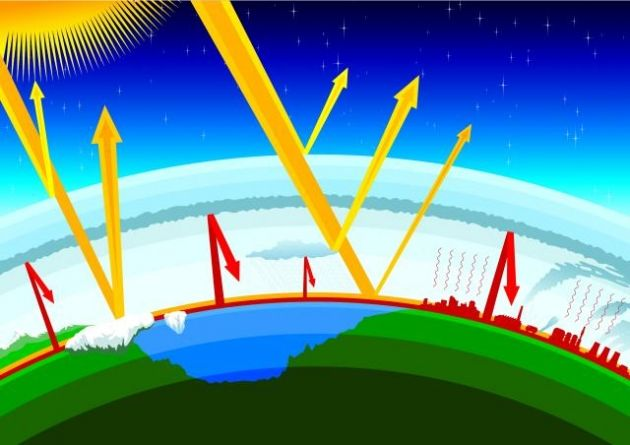
\includegraphics[width=0.7\linewidth]{imagenes/cap2/calentamientoGlobal}
			    	\caption{Calentamiento Global.}
			    	\label{fig:calentamientoGlobal}
			    \end{figure}
	\end{frame}
	
	%%%%%%%%%%%%%
	\subsection{Ciclo de carbono}
	\begin{frame}
		\frametitle{Ciclo de carbono}		
		\begin{figure}
			\centering
			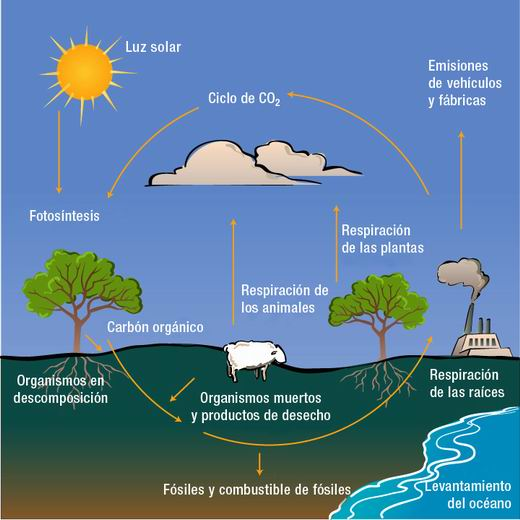
\includegraphics[width=0.5\linewidth]{imagenes/cicloCarbono}
			\caption{Procesos que componen el ciclo de carbono.}
			\label{fig:cicloCarbono}
		\end{figure}
	\end{frame}

	%%%%%%%%%%%%%
	\subsection{Secuestro de carbono}
	\begin{frame}
		\frametitle{Ciclo de carbono}		
		\begin{figure}
			\centering
			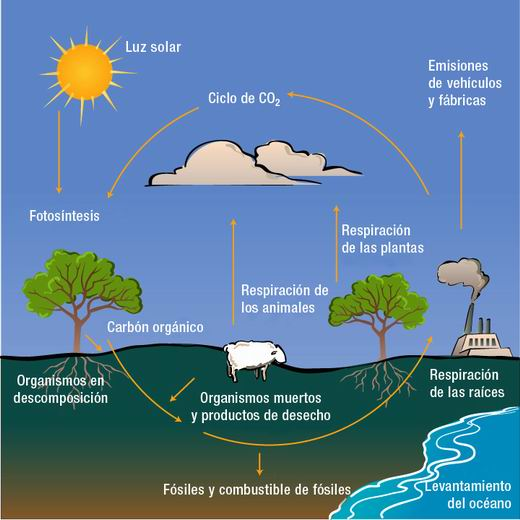
\includegraphics[width=0.5\linewidth]{imagenes/cicloCarbono}
			\caption{Procesos que componen el ciclo de carbono.}
			\label{fig:cicloCarbono}
		\end{figure}
	\end{frame}
	
		%%%%%%%%%%%%%
		\subsection{Medici\'on de balances de carbono}
		\begin{frame}
			\frametitle{Medici\'on de balances de carbono}		
			\begin{itemize}
				\item \textbf{Inventarios forestales.} 
				\begin{figure}[h!]
				\centering
				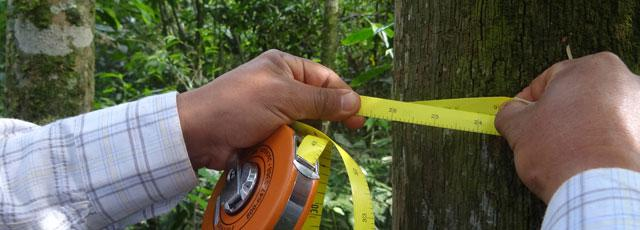
\includegraphics[width=0.7\linewidth]{imagenes/inventario-forestal}
				\label{fig:inventario-forestal}
				\end{figure}

				\item \textbf{Sensores remotos.} 
				\begin{figure}[h!]
				\centering
				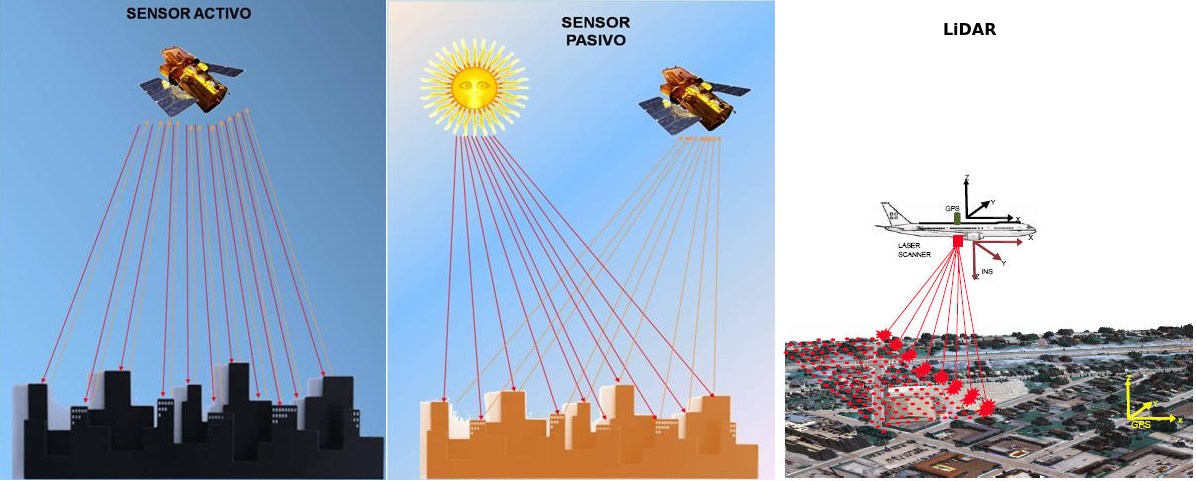
\includegraphics[width=0.7\linewidth]{imagenes/sensores}

				\label{fig:sensores}
				\end{figure}

			\end{itemize}
		\end{frame}

\end{document} 